\documentclass{article}

% Useful packages
\usepackage{multicol}
\setlength{\columnsep}{1cm}

% Set page size and margins
% Replace `letterpaper' with `a4paper' for UK/EU standard size
\usepackage[a4paper,top=2cm,bottom=2cm,left=2cm,right=2cm,marginparwidth=1.75cm]{geometry}

\usepackage{caption}
\usepackage{amsmath}
\usepackage{siunitx}
\usepackage{wrapfig}
\usepackage{float}
\usepackage{graphicx}
\graphicspath{{images/}}
\usepackage{subcaption}
\usepackage[colorlinks=true, allcolors=blue]{hyperref}
\usepackage{xcolor}
\usepackage{listings}
\usepackage{import}
\usepackage{xcolor}
\usepackage[toc,page]{appendix} % Pakket voor het maken van bijlagen
\usepackage{hyperref} % Pakket voor hyperlinks en verwijzingen

% Definieer de kleuren voor syntax highlighting
\definecolor{codegreen}{rgb}{0,0.6,0}
\definecolor{codegray}{rgb}{0.5,0.5,0.5}
\definecolor{codepurple}{rgb}{0.58,0,0.82}
\definecolor{backcolour}{rgb}{0.95,0.95,0.92}

\lstdefinestyle{mystyle}{
    backgroundcolor=\color{backcolour},
    commentstyle=\color{codegreen},
    keywordstyle=\color{codepurple},
    numberstyle=\tiny\color{codegray},
    basicstyle=\footnotesize\ttfamily,
    breakatwhitespace=false,
    breaklines=true,
    captionpos=b,
    keepspaces=true,
    numbers=left,
    numbersep=5pt,
    showspaces=false,
    showstringspaces=false,
    showtabs=false,
    tabsize=2
}

\usepackage[dutch]{babel}% Language setting


\title{Aandrijftechniek Moonrover}

\author{
  Vollmuller, Michel\\
  1809572\\
  \texttt{michel.vollmuller@student.hu.nl}
  \and
  Willems, Tijmen\\
  1805057\\
  \texttt{tijmen.willems@student.hu.nl}
}

\begin{document}
\maketitle

\begin{abstract}
    Hier komt een mooie abstract
\end{abstract}

\tableofcontents

\newpage

\section{Inleiding}
De Euro Moon Rover is een compact, wendbaar voertuig ontworpen voor het verkennen van het maanterrein. Met zijn vier individueel aangestuurde wielen kan het obstakels tot de grootte van de radius van het wiel overwinnen. Het voertuig is snel en robuust, uitgerust met gelijkstroommotoren van Maxon die zijn aangepast om te functioneren in de extreme omstandigheden van de maan. Dankzij zijn ontwerp en aanpassingen is de Euro Moon Rover goed uitgerust om wetenschappelijke missies uit te voeren en het oppervlak van de maan te verkennen.


\section{Analyze} 
\subsection{Vraagstelling}
\textbf{Hoofdvraag:}
Is de door Maxon voorgestelde aandrijving de beste oplossing voor de Euro Moon Rover?\\
\textbf{Deelvragen:}
\begin{enumerate}
    \item Wat zijn de lasten en wat zijn de wensen?
    \item Wat is de juiste mechanische transmissie?
    \item Wat zijn de juiste specificaties voor de motor?
    \item Wat is de efficientie van de motor?
\end{enumerate}

\subsection{Specificaties}
\begin{align*}
  \textbf{Moonrover}\\
  &\text{Gewicht :} & 6 \, \text{kg} \\
  &\text{formaat (lengte*breedte):} & 40*25 \, \text{cm}\\
  \textbf{Wielen}\\
  &\text{diameter wielen :} & 15 \, \text{cm}\\
  &\text{wrijvingscoefficient :} & 0.9 \, \\
  &\text{rolweerstandcoefficient :} & 0.1 \, \\
  &\text{Massatraagheid (J) :} & \text{$2.1 \cdot 10^{-3}$} \, \text{$kg \cdot m^{2}$}\\
  \textbf{Eisen / Wensen}\\
  &\text{topsnelhied vlakke grond :} & 2.1 \, \text{$m/s$}\\
  &\text{versnelling vlakke grond :} & 0.7 \, \text{$m/s^{2}$}\\
  &\text{vertraging vlakke grond :} & 0.5 \, \text{$m/s^{2}$}\\
  &\text{max helling :} & 30 \, \text{degrees}
\end{align*}

\newpage

\section{Lasten}
In dit hoofdstuk worden de verschillende lasten van de moonrover berekend. In de formules word er een hellingshoek aan gehouden van 0 graden. De bescreven fomrules zijn allemaal voor 1 wiel. Voor de gehele moonrover zal dit dus x4 moeten. In de afbeeldingen is ook te zijn hoe de eigenschappen zich gedragen onder diverse hellingshoeken.

\subsection{Rollast}
    Rollast is de last die minaal overwonnen moet worden een wiel te laten draaien. Dit verschilt ook onder welke hellingshoek de moonrover staat. In afbeelding \ref{fig:birds} is te zien hoe de rolllast veranderd onder diverse hellingshoeken.

    \begin{figure}[H]
        \centering
        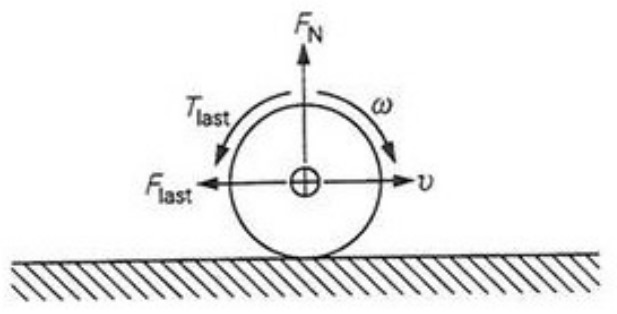
\includegraphics[scale=0.5]{Rolweerstand.jpg}
        \caption{rollast krachten}
    \end{figure}

    \begin{multicols}{2}
        \textbf{Formules:}
        \begin{equation}
            \begin{split}
                T_{last} &= f_{rol} \cdot F_{N} \cdot r \\
                F_{N} &= m \cdot g \cdot cos(\alpha) \\
                &\Downarrow \\
                T_{last} &= 0.1 \cdot 2.43 \cdot 0.075 = 18.23 [mNm]
            \end{split}
        \end{equation}

        \textbf{constante:}
        \begin{equation*}
            \begin{split}
                f_{rol} &= 0,1 \\
                r &= 0,075 [m] \\
                m &= 1,5 [N] \\
                g &= 1,62 [m/s^2] \\
                \alpha &= 0^\circ
            \end{split}
        \end{equation*}
    \end{multicols}

\subsection{Hellingslast}
    Hellingslast is de last die om de hoek komt kijken zodra de moonrover zich onder een helling bevindt. Wanneer deze helling stijgend is zal dit de last zijn die overtroffen moet worden om voorruit te komen. Wanneer deze helling dalend is is dit de last die overtroffen moet worden of tot stilstand te komen.

    \begin{figure}[H]
        \centering
        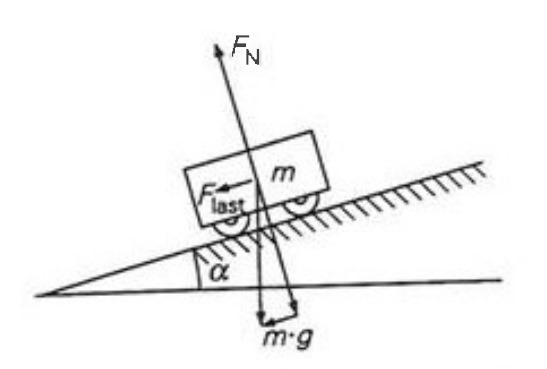
\includegraphics[scale=0.5]{Hellingsweerstand.jpg}
        \caption{hellinglast krachten}
    \end{figure}

    \begin{multicols}{2}
        \textbf{Formules:}
        \begin{equation}
            \begin{split}
                T_{last} &= f_{N} \cdot sin(\alpha) \cdot r \\
                F_{N} &= m \cdot g \cdot cos(\alpha) \\
                &\Downarrow \\
                T_{last} &= 2.43 \cdot 0 \cdot 0.075 = 0 [mNm]
            \end{split}
        \end{equation}

        \textbf{constante:}
        \begin{equation*}
            \begin{split}
                r &= 0,075 [m] \\
                m &= 1,5 [N] \\
                g &= 1,62 [m/s^2] \\
                \alpha &= 0^\circ 
            \end{split}
        \end{equation*}
    \end{multicols}

    \begin{figure}[H]
        \centering
        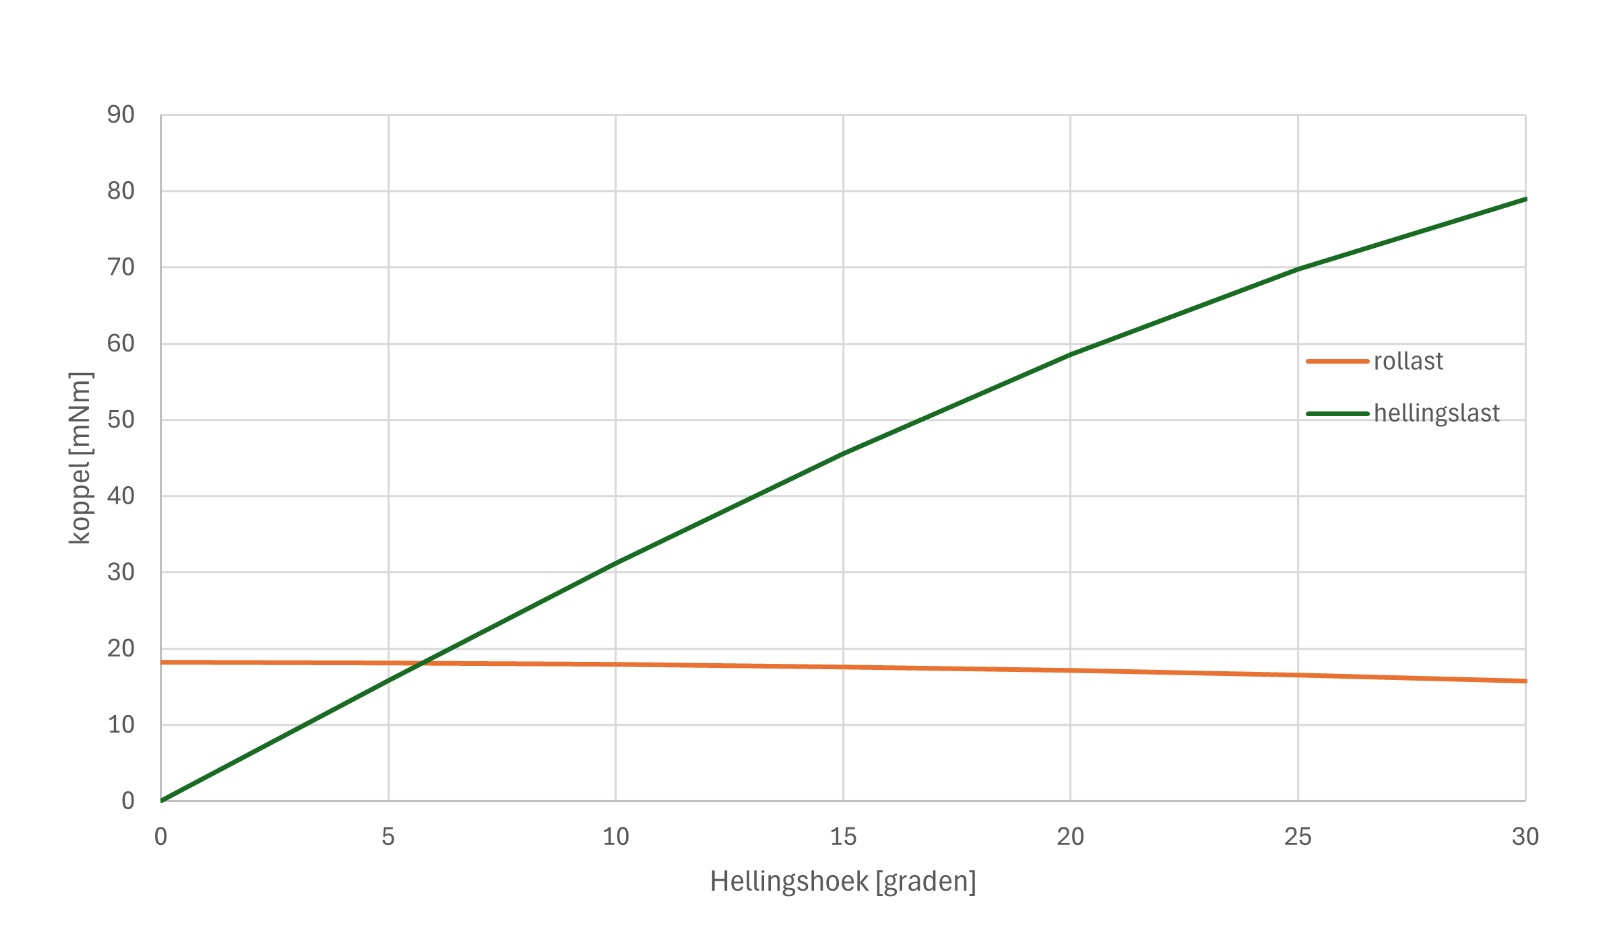
\includegraphics[scale=0.3]{grafiek hellingsweerstand en rolweerstand.jpg}
        \caption{rolweerstand vs hellingsweerstand onder verschillende hoeken}
        \label{fig:birds}
    \end{figure}

    In figuur \ref{fig:birds} is te zien hoe de rolweerstand en de hellingsweerstand zich gedragen ten opzichte van verschillende hellingshoeken. In de grafiek is te zien dat vanaf een hoek $\approx 5.7^\circ$ de moonrover altijd stil zal blijven staan. Dit komt doordat de moonrover tot dit punt nog niet voorbij zijn rollast komt. Het snijpunt van de rollast met de hellingslast wordt als volgt berkent:
    \begin{equation}
        \begin{split}
            T_{rollast} &= T_{hellingslast} \\
            f_{rol} \cdot F_{N} \cdot r &= F_{N} \cdot sin(\alpha) \cdot r \\
            f_{rol} &= sin(\alpha) \\
            0.1 &= sin(\alpha) \\
            \alpha &= sin-1(0.1) \\
            \alpha &= 5.72^\circ
        \end{split}
    \end{equation}

\subsection{Grip}
    Onder grip verstaan we de hoeveelheid torque die op de aandrijving gegeven kan worden zonder dat het wiel zal gaan slippen. Hierbij berkenen we dus ook wat de maximale torque is die gegeven kan worden op de aandrijving.

    \begin{multicols}{2}
        \textbf{Formules:}
        \begin{equation}
            \begin{split}
                T_{max} &= \mu \omega \cdot F_{N} \cdot r \\
                F_{N} &= m \cdot g \cdot cos(\alpha) \\
                &\Downarrow \\
                T_{max} &= 0.9 \cdot 2.43 \cdot 0.075 = 164.03 [mNm]
            \end{split}
        \end{equation}

        \textbf{constante:}
        \begin{equation*}
            \begin{split}
                \mu \omega &= 0.9 \\
                r &= 0,075 [m] \\
                m &= 1,5 [N] \\
                g &= 1,62 [m/s^2] \\
                \alpha &= 0^\circ 
            \end{split}
        \end{equation*}
    \end{multicols}

    \begin{figure}[H]
        \centering
        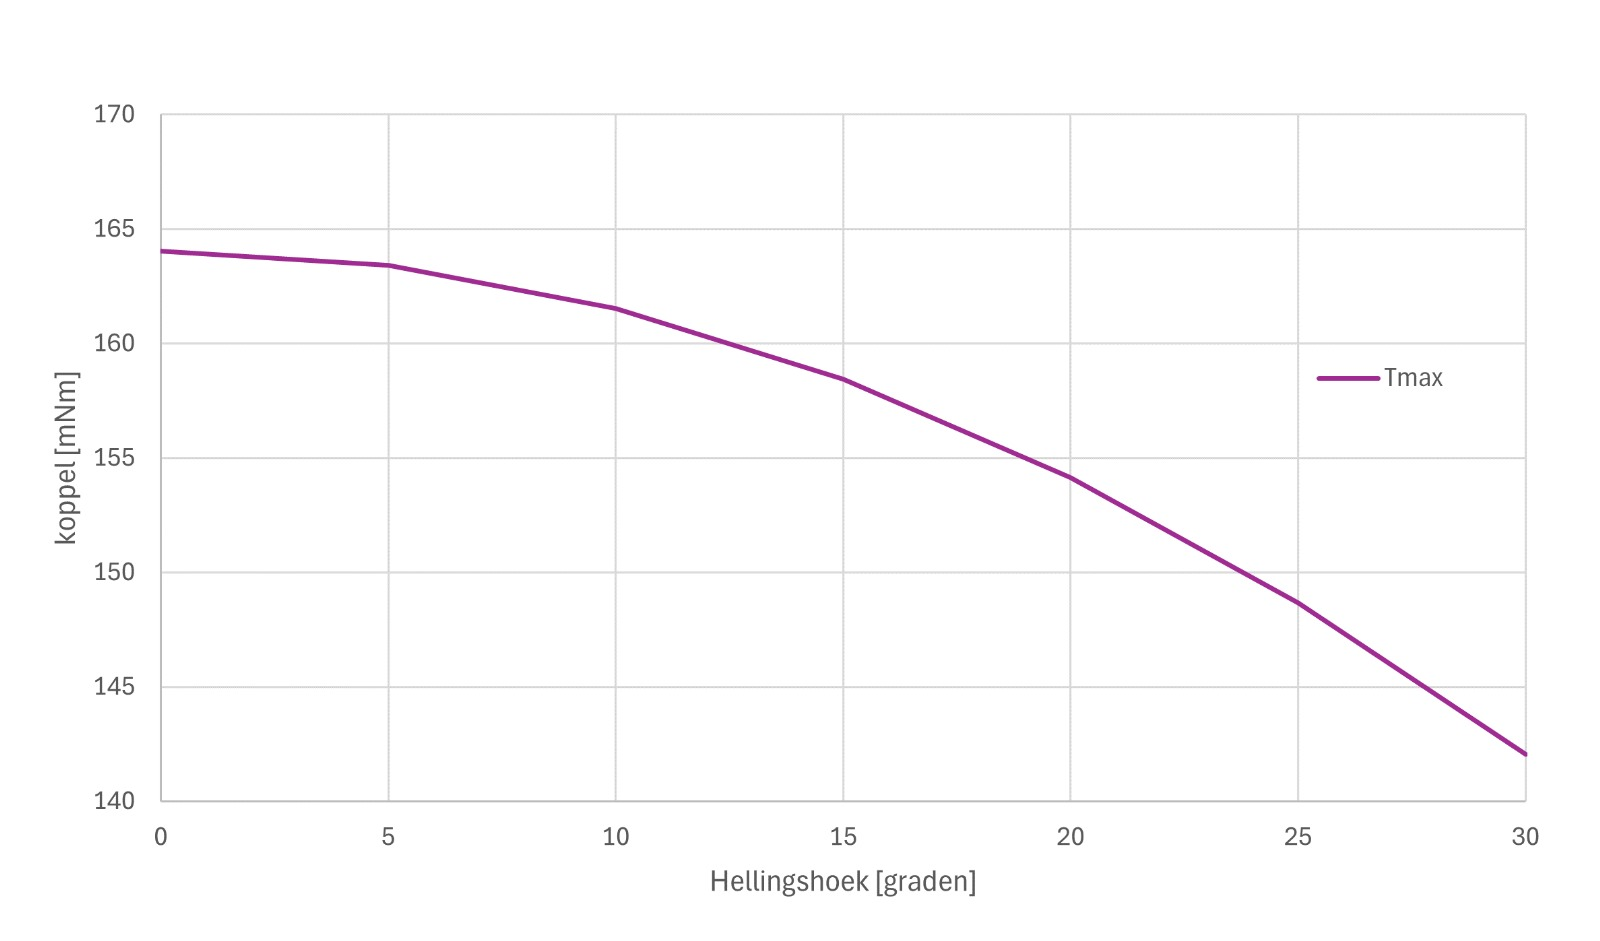
\includegraphics[scale=0.3]{grafiek max koppel.jpg}
        \caption{$T_{max}$}
        \label{fig:peanut}
    \end{figure}

    In figuur \ref{fig:peanut} is te zien hoe de maximale koppel zich weerhoud tegen de hellingshoek. Hierbij is duidelijk te zien dat de maximale koppel af neemt naarmate de hellingshoek groter wordt.

\subsection{Versnelling}
    Hier wordt het koppeloverschot berkend wat nodig is om de beoogde versnelling te behalen. 

    \begin{multicols}{2}
        \textbf{Formules:}
        \begin{equation}
            \begin{split}
                T_{acc} &= J \cdot \frac{d \omega}{dt} \\
                omtrek_{wiel} &= 2 \cdot \pi \cdot r = 0.47 [m] \\
                Versnelling &= \frac{a}{omtrek_{wiel}} = 1.49 [omwentelingen/s^2] \\
                &= 9.36 [rad/s^2] \\
                &\Downarrow \\
                T_{acc} &= 2.1 \cdot 10^{-3} \cdot 9.36 = 19.6 [mNm]\\
            \end{split}
        \end{equation}

        \textbf{constante:}
        \begin{equation*}
            \begin{split}
                a &= 0.7 [m/s^2] \\
                J &= 2.1 \cdot 10^{-3} [kg \cdot m^2]\\
                r &= 0,075 [m] \\
                m &= 1,5 [N] \\
                g &= 1,62 [m/s^2] \\
                \alpha &= 0^\circ 
            \end{split}
        \end{equation*}
    \end{multicols}

\subsection{Snelheid}
    Hier berkenen we de maximale rpm waarbij de maximale snelheid van van 2.1 m/s niet word overtroffen.

    \begin{multicols}{2}
        \textbf{Formules:}
        \begin{equation}
            \begin{split}
                omtrek &= 2 \cdot \pi \cdot r \\
                snelheid &= \frac{speed_{max}}{omtrek}\ = \frac{2.1}{0.47} = 4.46 [omw/s]\\
                &\Downarrow \\
                 &= 267.4 [rpm]
            \end{split}
        \end{equation}

        \textbf{constante:}
        \begin{equation*}
            \begin{split}
                speed_{max} &= 2.1 [m/s]\\
                r &= 0,075 [m] 
            \end{split}
        \end{equation*}
    \end{multicols}

\newpage

\subsection{Conclusie}
In dit hoofdstuk heb je kunnen lezen hoe we de lasten van de moonrover hebben bepaald. Dit was nodig om een geschikte motor te selecteren voor de moonrover.  In afbeelding \ref{fig:lasten moonrover} is het werkgebied te zien van de moonrover doormiddel van de rode lijnen. In het volgnende hoofdstuk zal er een geschikte motor en transmissie geselecteerd worden die juist aansluit bij deze last. 

\begin{figure}[H]
    \centering
    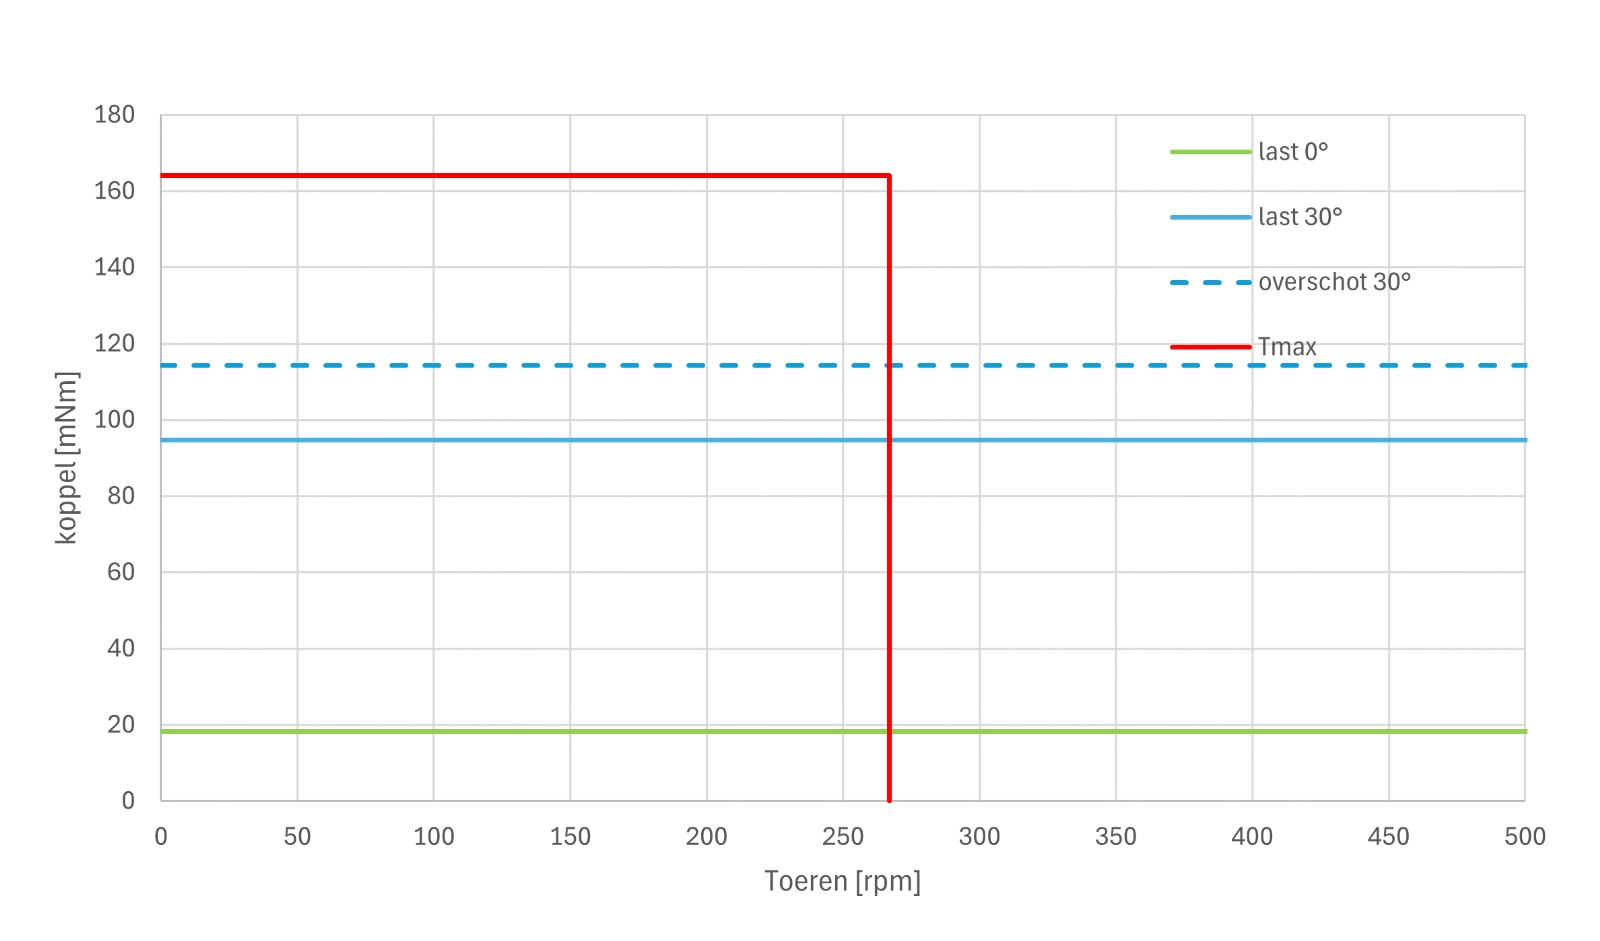
\includegraphics[scale=0.3]{last conclusie.jpg}
    \caption{Lasten moonrover}
    \label{fig:lasten moonrover}
\end{figure}
    


\newpage

\section{Motor}
In het volgende hoofdstuk is zijn de lasten van de moonrover bepaald. Op basis van deze gegevens kunen we de juiste motor gaan selecteren voor de moonrover. Door de leverancier "Maxon" is er een advies gedaan van een reeks motoren en transmissies;
\begin{align*}
        motor: &RE25 1187xx\\
        transmissie: &Planetary Gearhead GP xx xx
\end{align*}
In dit hoofdstuk zullen wij een keuze gaan maken voor een specifieke motor in combinatie met een specifieke transmissie.


\subsection{Motorkeuze}
Binnen de aangegeven maxon reeks hebben wij gekozen voor de RE25 118745. In theorie is het mogelijk om elke motor te kieze binnen de aangegeven reeks in combinatie met de juiste transmissie. Voor deze specifieke situatie hebben we gekozen voor de RE25 118745. Dit is een wat kleinere motor binnen de reeks, echter is het mooie van deze motor dat hij een efficientie van 90 heeft. In afbeelding \ref{fig:RE25_118745} is te zien hoe de koppel toeren karakteristiek van de motor zich weerhoud tegen de last. In combinatie met de juiste transmissie kan deze motor goed ingezet worden bij de moonrover. In Bijlage \ref{app:datasheet motor} is de datasheet te zien van deze motor.
\begin{figure}[H]
        \centering
        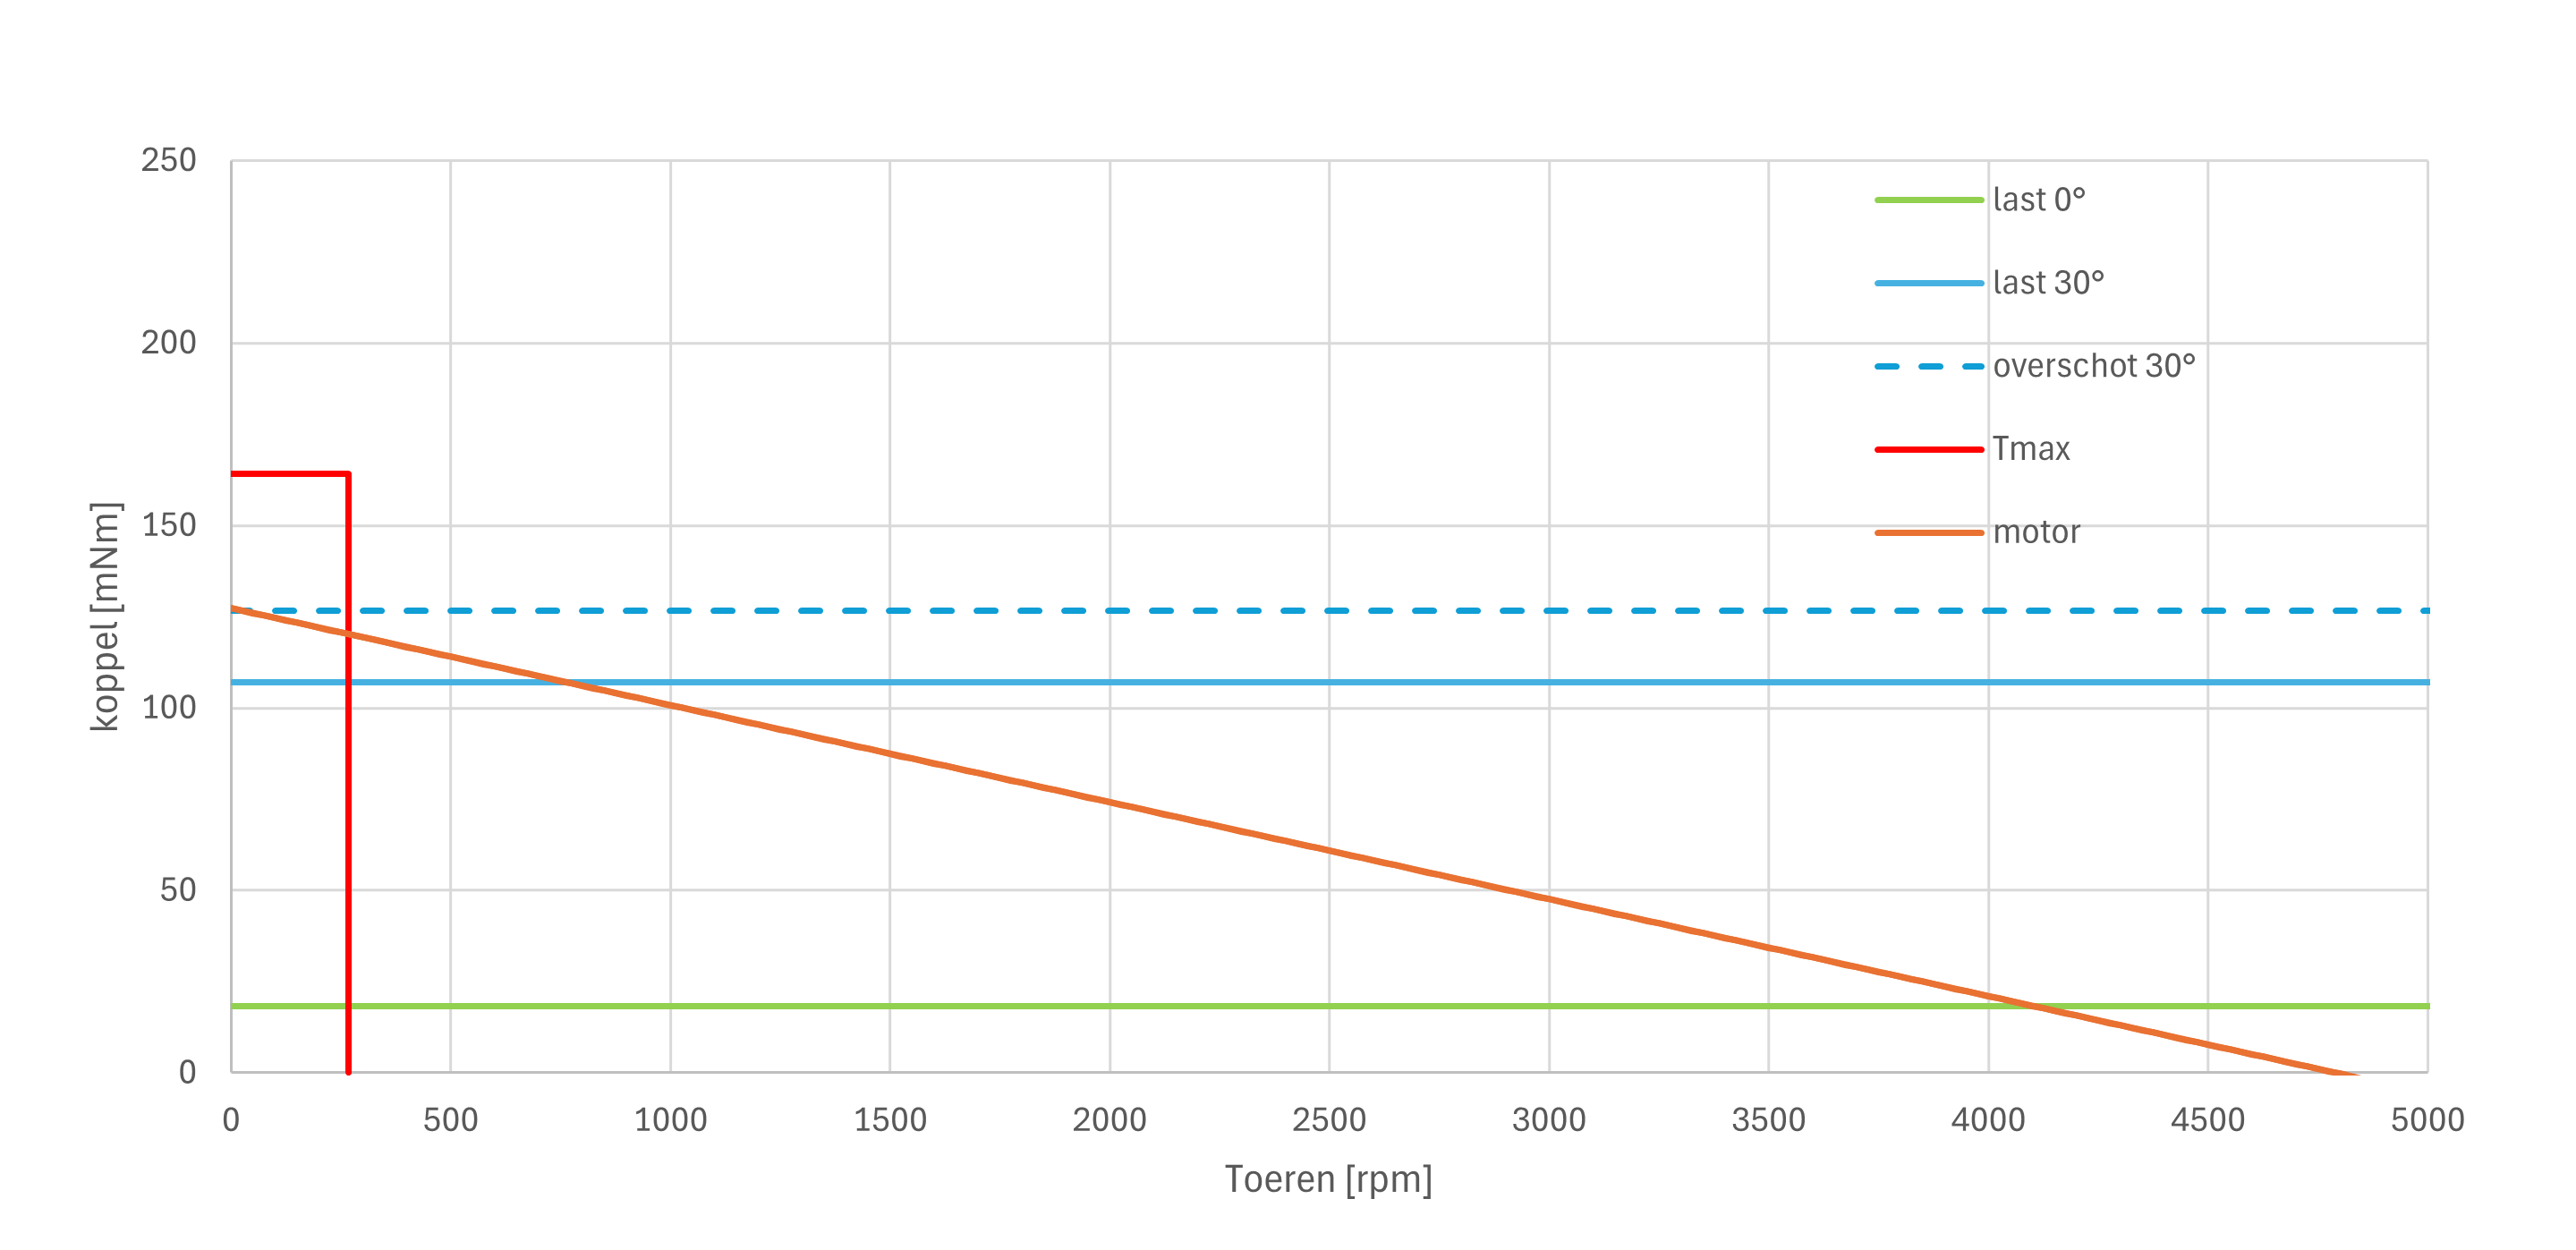
\includegraphics[scale=0.7]{RE25_118745.png}
        \caption{koppel toeren karakteristiek RE25 118745}
        \label{fig:RE25_118745}
    \end{figure}

\subsection{transmissiekeuze}

\subsection{efficientie}



\subsection{Warmtedisipatie}

Voor de moonrover zullen de motoren geleverd worden van het merk Maxon. Maxon heeft aangegeven dat zij de gekozen motor "maan bestendig" zullen maken. Hierbij zal ook rekening gehouden met de temperatuur verschillen op de maan en de warmte dissipatie hiervan. 

\subsection{Conclusie}
% Motor kromme berekennen
% motor kromme laten zien en uitleggen
% rendement bereken
% efficientie
% warmte

\newpage

\section*{Conclusie}
Het onderzoek naar de aandrijftechniek van de moonrover heeft geleid tot de selectie van de RE25 118745 motor in combinatie met de Planetary Gearhead GP 32 A 166158 transmissie. De keuze voor deze motor is gebaseerd op zijn efficiëntie van 90\%, wat gunstig is voor de prestaties van de moonrover. De transmissie is essentieel gebleken om het maximale koppel te behalen en de motor rond zijn nominale toerental te laten werken. De berekende totale efficiëntie van 67,5\% benadrukt het belang van het optimaliseren van zowel de motor als de transmissie voor een effectieve aandrijving van de moonrover. In conclusie biedt dit onderzoek een solide basis voor de verdere ontwikkeling en implementatie van de diverse componenten in de moonrover, met een focus op efficiëntie, prestaties en betrouwbaarheid in een uitdagende omgeving.

%Bibliography
% \bibliographystyle{IEEEtran}
% \bibliography{bib}
% \appendix

% \bibliographystyle{IEEEtran}
% \bibliography{bib}

\newpage
% Bijlage's    
\begin{appendices}

\section{Datasheet RE25 118745}
\label{app:datasheet motor}
\begin{figure}[htbp]
  \centering % trim=left bottom right top
  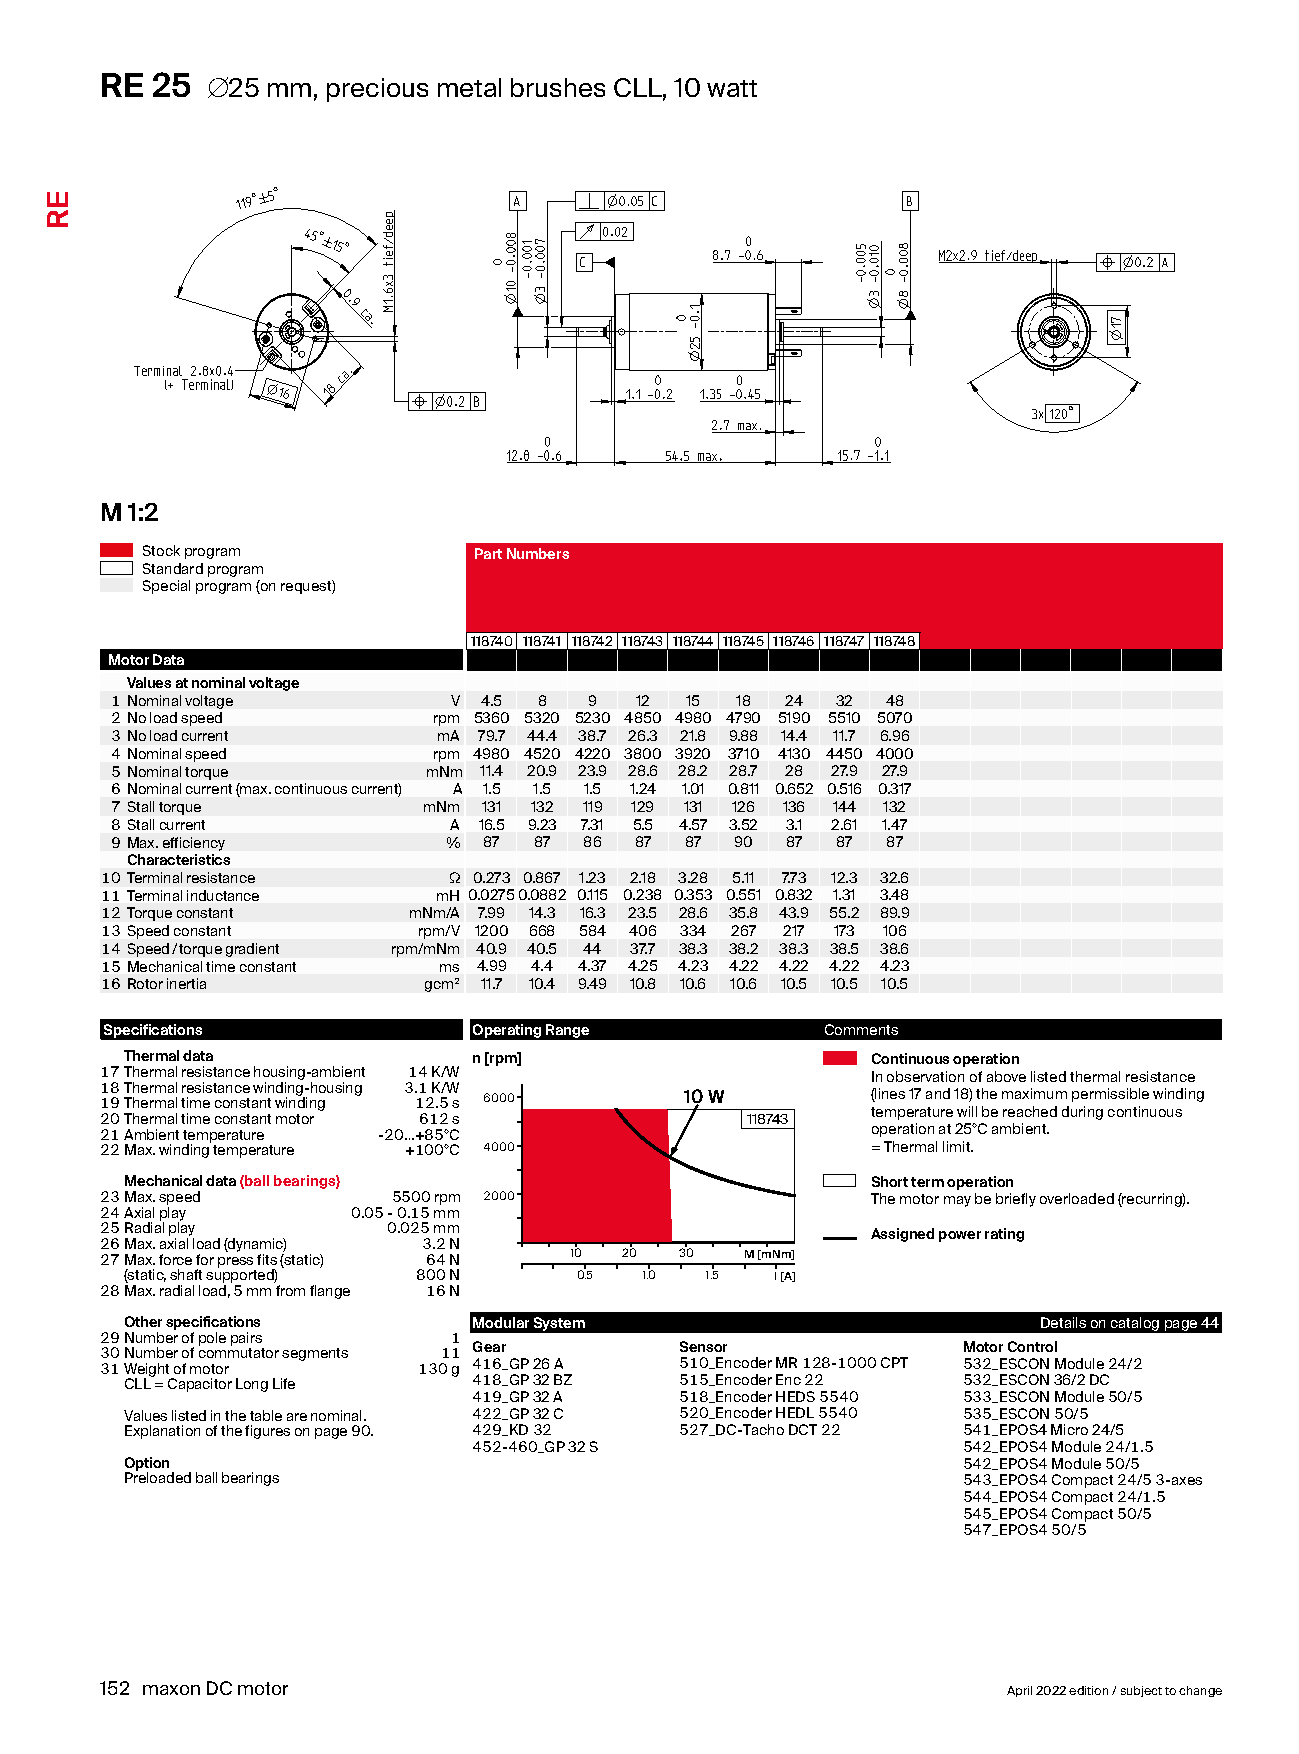
\includegraphics[page=1, clip, trim=0cm 0cm 0cm 0cm, scale = 0.65]{datasheet_RE25118745.pdf}
  \caption{datasheet RE25 118745}
  \label{fig:datasheet RE25 118745}
\end{figure}

\newpage

\section{Datasheet Planetary Gearhead GP 32 A 166158}
\begin{figure}[htbp]
  \centering % trim=left bottom right top
  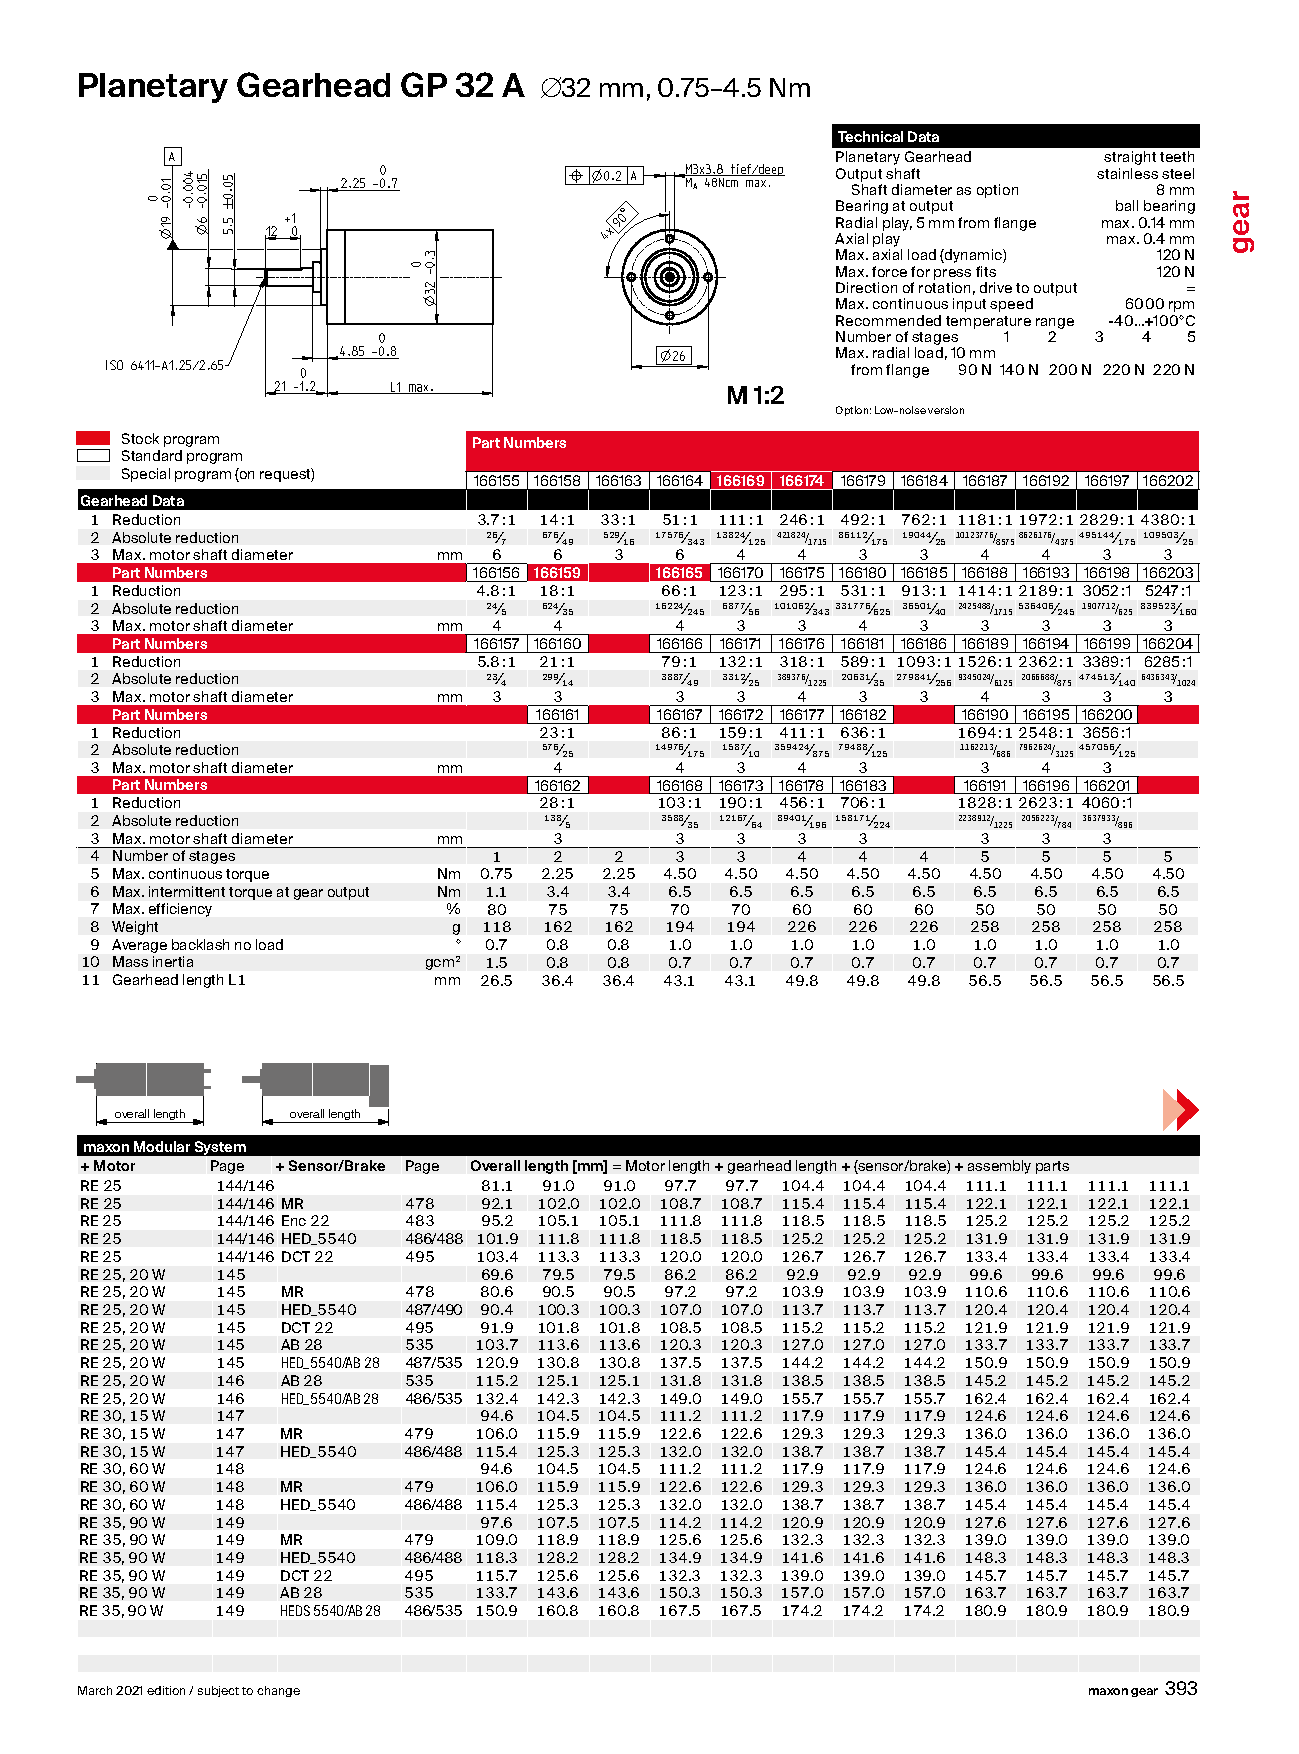
\includegraphics[page=1, clip, trim=0cm 0cm 0cm 0cm, scale = 0.65]{datasheet Planetary Gearhead GP 32 A 166158.pdf}
  \caption{datasheet Planetary Gearhead GP 32 A 166158}
  \label{fig:datasheet Planetary Gearhead GP 32 A 166158}
\end{figure}

\end{appendices}

\end{document}